% Chapter 

\chapter{Artefact Evaluation} % Main chapter title

\label{Chapter9_artefact-evaluation} % For referencing the chapter elsewhere, use \ref{Chapter9} 

\section{Introduction }
This chapter is about the evaluation process of the work done in section \ref{New artefact prototype} in  chapter \ref{Chapter8_artefact-design}, \nameref{Chapter8_artefact-design}  to create the artefact \enquote{Cybernewsfeed Technology}. The relevance of the created artefact \enquote{Cybernewsfeed Technology} is validated by the Focus Group and the approach and outcome of the validation process is explained in this chapter.

\section{Evaluation Process}
As mentioned in chapter \ref{Chapter6_research-approach} \nameref{Chapter6_research-approach}, this research was designed to perform validation using Group Support System (GSS) under the Design Science Research (DSR) framework. 
For the validation of artefact, this thesis took focus group
\citep{langford2012qualitative} discussion approach for GSS. 
To run the GSS validation,
it was needed to have a focus group
\citep{langford2012qualitative} 
of six to eight people with similar background in the cybersecurity threat intelligence domain and who are willing to uncover a range of perspectives and experiences. 
The shortlisted  focus group participants as per list of Appendix \ref{AppendixChapter9}, \nameref{AppendixChapter9}
 were invited to participate in the group session. 
The pre-read materials, scope, agenda and presentation to be used during the session were shared upfront with the participants. 
The session was scheduled on 15th July 2020, 
Wednesday between 18:00 to 20:00 hours via an online Zoom meeting with the help of experienced moderators who captured the broad range of views of the group.


\subsection{Scope and Objective}
The scope of this Group support system research was to demonstrate and validate the prototype which had been build. 
This group session took approximately two hours, 
starting with prototype demo and  presentation.
 After that an open discussions about the design and functionality of the artefact among the focus group. 
In the end we ran an online survey to let the Focus group share the expertise, 
perspective and experience on the topic.

\subsubsection{Objectives of the session}
\begin{itemize}
    \item Primary objective is to examine the automated Cybernewsfeed tooling modules that collects,
ingests and parses relevant cyber information based on adjustable parameters.
    \item Secondary objective of the survey is to get insight on the form, frequency, pricing and content of such a cybernewsfeed Brief.
\end{itemize}

\subsubsection{Survey type}
I have made use of GSS because GSS is very craftful for making use of experts or focus group of people that are geographically spread but can attend physically. Choosing a Group system support(Focus group) mechanism ensured that participants represented all the three levels of stakeholders to discuss on the topic of \enquote{Cybernewsfeed Technology}. During the Focus Group discussion, we captured the responses of Focus Group participants using Meeting Wizard\footnote{\url{https://www.meetingwizard.nl/}} tool and the professor Yuri Bobbert who is specialised in GSS was the moderator of this session. The GSS session was observed by Willy Lund\footnote{An ON2IT facilitator} so that the execution of GSS session goes according to the academic principles. 

\subsubsection{Agenda}
The Agenda set for two hours for the GSS was structured as below.

\begin{itemize}
    \item The artefact prototype Expectation Setting - 5 Min
    \item Understanding The Prototype - 15 Min
    \item Open Discussion by Focus group about the prototype - 15 Min
    \item Demo: Cybernewsfeed Technology(The Artefact) - 15 Min
    \item Survey: To collect Focus group opinion - 70 Min
\end{itemize}

\subsubsection{Demo Link}\label{Demo Link}
In the link below, you can find the demo video of the tool which is a pre-recording of the tool \enquote{Cybernewsfeed Technology}. This demo video was presented to the Focus group.
\begin{itemize}
    \item \url{https://drive.google.com/file/d/1P8eFg7wJtW55Z3QfAO8qCHbZJqlao9Q6/view?usp=sharing}
\end{itemize}



\subsubsection{Survey Questions in GSS}
\begin{enumerate}
    \item What is the industry that you are working in? (Brainstorm)
    \item At what level are you positioned in your organisation? (Flipboard)
    \item At what level are you positioned in your organisation? (Voting)
    \item How would you rate the quality? (Flipboard)
    \item How would you rate the quality of the end product? (Voting)
    \item Requirement setting. (functional and technical) (Brainstorm)
    \item What is your experience with such a technology? (Flipboard)
    \item What is your experience with a Cybernewsfeed technology? (Voting)
    \item How interested are you in such a cyber newsfeed? (Flipboard)
    \item Please rate your interest in such a cyber newsfeed. (Voting)
    \item Ordering of the cyber newsfeed content items' relevance. (Flipboard)
    \item Relevance of the cyber newsfeed content (what is your preference?) (Voting)
    \item Frequency of the Cybernews feed. (Flipboard)
    \item Selecting the frequency of the cyber newsfeed. (Voting)
    \item Media form of the cyber newsfeed. (how to receive) (Flipboard)
    \item Selecting the media form. (Voting)
    \item Pricing range of the cyber newsfeed technology. (Flipboard)
    \item Pricing of the Cybernewsfeed technology + advisory. (Voting)

\end{enumerate}

\section{Artefact Evaluation Results}\label{Artefact Evaluation Results}
In this section we have mentioned the collected feedbacks about the artefact \enquote{Cybernewsfeed Technology}. These feedbacks higlights about the following two things: 1) participant's familiarity with the similar product and 2) demand and desire of the cybernews brief created via such a cybernews feed technology. The parameters for GSS evaluation are mentioned in the survey questions.  We have also captured additional functional and technical requirements for the next iteration of the artefact development.

\subsection{Representation and Background of Participants of the Focus group}
This section reflects the answer to the survey question number one, two and three. It showed that the Focus group represents four different industries:
\begin{enumerate}
    \item Healthcare
    \item Finance
    \item Government
    \item Chemical
\end{enumerate}
 About the background of the participants, the participants in the group were functional as stakeholders at multiple levels:
 \begin{itemize}
     \item Tactical/Management: 3
     \item Strategic/Board: 6
     \item Operational: 2
 \end{itemize}
\subsection{Additional functional and technical requirements}
This section lists the answers to the survey question number six, where participants expects additional functionalities on the top of existing functionalists in the demo artefact. Participants shared these following  functional and technical requirements.
\begin{enumerate}
    \item Additional technical requirements you would like to see/have?
    \begin{enumerate}
        \item Decision tree info on the level of filtering.
\item Ranking of cyber newsfeed items. 
\item  Risk Rating of Vulnerabilities.
\item  Expected complexity to implement.
\item  Maintenance of the decision tree.
\item Continuous monitoring and reporting of new vulnerabilities.
\item  Relevance (higher/lower) in terms of relevance to the existing landscape, processes, policies, risk appetite etc.
\item  Technical value score of software supplier (past).
\item  The current and trending hot topics in cyber world. 
\item  Information about the RTO\footnote{RTO \url{https://en.wikipedia.org/wiki/Disaster_recovery\#Recovery_Time_Objective}}, RPO\footnote{RPO \url{https://en.wikipedia.org/wiki/Disaster_recovery\#Recovery_Point_Objective}} and Availability in case of known security incidents.

\item Reliable and secure information sources.
\item Add  information relating to OWASP\footnote{Open Web Application Security Project (OWASP)\url{https://en.wikipedia.org/wiki/OWASP} }, SANS25\footnote{SANS\footnote{\url{https://en.wikipedia.org/wiki/SANS_Institute}} top Top 25 Software Errors\url{https://www.sans.org/top25-software-errors}}, General Data Protection Regulation (GDPR)\footnote{\url{https://en.wikipedia.org/wiki/General_Data_Protection_Regulation}} , ISO27001 and various other legal requirements.
    \begin{itemize}
        \item Reference, if the vulnerability relates to elements in these domains. Related to if an organisation has to adhere to any of these
        principles.
     \item How will patch updates if any be performed?
    \end{itemize}

\end{enumerate}
    \item Additional functional requirements you would like to see/have?
    \begin{enumerate}
        \item Dashboard on supplier, vulnerability history and speed of solving.
        \item Role based management (managing info supply).
        \item Ability to customize / filter feeds based on "need to know" and "nice to know / trend" information.
        \item Ability to list and rank data sources.
    \end{enumerate}
\end{enumerate}


\subsection{Prototype Demo feedback}
 The artefact demo video of 15 minutes was played to show the end-to-end functionalities of the Collector, of the Processor and of the Analyser \& Advisory modules. 
The general feedback of the Focus group participants were positive and the concept of making such a prototype was rated as new. 
Some comments captured from Focus group participants is shown in FIGURE \ref{fig:feedback}.

\begin{figure}[ht]
    \centering
    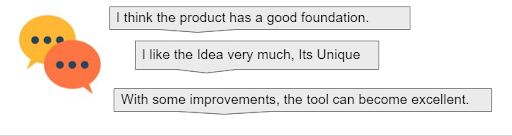
\includegraphics[width=.65\linewidth]{Figures/feedback.png}
    \caption{Focus group Comments on the artefact demo}
    \label{fig:feedback}
\end{figure}
 \FloatBarrier

\subsection{Familiarity with such product}
\label{ref:familiar}
This was the reflection of the survey question number seven and eight. All the participants in the Focus group were familiar with similar technology and some of them have already used. 
There was no one who is not aware of cyber intel technology. 
Participants familiarity with such technology ensured that the validation process in on right track and everyone understands, and can respond to the questions related to the demo product. In FIGURE \ref{fig:product-familarity}, the pie chart representation of the individual responses from the participants is shown.

\begin{figure}[ht]
    \centering
    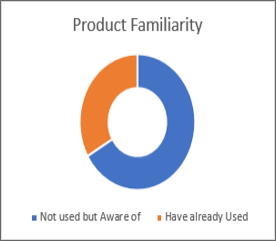
\includegraphics[scale=0.6]{Figures/product-familarity.png}
    \caption{Familiarity: Group Knowledge on similar technology }
    \label{fig:product-familarity}
\end{figure}
 \FloatBarrier

\subsection{Interest in such product}
\label{sec:interest}
This was the reflection of the survey question number nine and ten. Here I have checked the interests of the group for such a product and the results were very interesting. 
Half of the group was slightly interested 
and the other half were very interest. 
There was no one from the group who was not interested in such a product. 

\begin{figure}[ht]
    \centering
    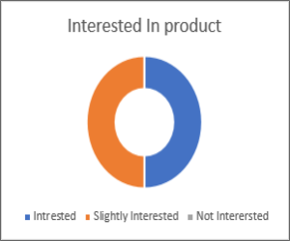
\includegraphics[scale=0.6]{Figures/product-interest.png}
    \caption{Interest: in similar technology}
    \label{fig:product-interest}
\end{figure}
 \FloatBarrier

\subsection{About the product concept}
\label{sec:concept}
 The topic of survey questions four and five was the validation of the product concept. 
 The questions where answered by selection one of the following options: Excellent, Good, Average or Poor. 
 In addition to the voting option there was a text field available for additional feedback. 
 Of the six participants three (50\%) voted `Good` and three (50\%) voted `Average` 
 (See FIGURE \ref{fig:product-concept}).
The free text feedback of the six participants
is included below.

%This was the reflection of the survey question number 4 and 5. For validating the product concept, we used voting options and captured the additional information as text.
%According to the responses captured from the participants based on the rating of Good, Average, Excellent or Poor, here is the list. The group's comments has been presented in its format before the reader.

\begin{figure}[ht]
    \centering
    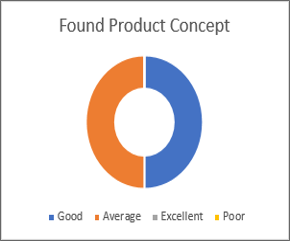
\includegraphics[scale=0.6]{Figures/product-concept.png}
    \caption{Concept: About the artefact demo during GSS}
    \label{fig:product-concept}
\end{figure}
 \FloatBarrier

 \begin{enumerate}
 \item Good
 \begin{enumerate}
\item Missing rating of the reported data. Also what is the quality of this reported data. This information will improve
this tool further.
\item Based on the limited amount of information so far I thing the product has a good foundation. I see however some
improvements in the contextualization of the information on operational level (maybe mapping against a CMDB). I
also suggest a feedback loop (measures the effectiveness and quality of the risk mitigation/information put in
context) and the risk assessment (probability, risk level, Vulnerability, Impact, Frequency) and prioritization of risk
mitigating actions proposed by the tool.
\item Filling in the raw data based on the short data seems like it could become a strenuous task, especially with
multiple sources. 
\\- Add a list of possible sources based on their quality rating and information. 
\\- Including and
elements related to the Look and feel and intuitive design are important
  \end{enumerate}
   \item Average 
   \begin{enumerate}
      
  
    \item Decision tree role based advice (agile) just in time (if i'm developing other feed is needed than in Production)
 \item The decision tree is key for the value of the tool. that will make the tool good. With improvements on the
reporting part, considering risks, prioritisation and stakeholder management, the tool can become excellent.
 \item Can consist of some additional requirements for follow up of actions, prioritization, branch specific information,
continuous run that presents me actionable information as soon as it becomes available. The UX should be way better. Do not invite me to use with this GUI.
 \end{enumerate}
   \item Excellent 
   \begin{enumerate}
       \item Not Applicable 
   \end{enumerate}
   \item Poor
   \begin{enumerate}
       \item Not Applicable 
   \end{enumerate}
 \end{enumerate}



\subsection{Desired cyber newsfeed type}
\label{sec:desire}
This was the reflection of the survey question number 11 and 12. In this section, we captured the newstype by priority for the type of news listed in TABLE \ref{tab:stakeholder-news}. 
The group's interested and their comments in as it is format has been presented before the reader. In FIGURE \ref{fig:product-desire}, the desired cyber newsfeed type is listed by priority.

\begin{figure}[ht]
    \centering
    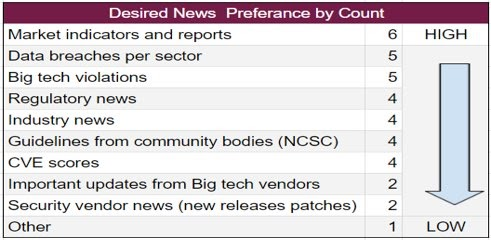
\includegraphics[width=.75\linewidth]{Figures/product-desire.jpg}
    \caption{Desired cyber newsfeed type: Priority high to low}
    \label{fig:product-desire}
\end{figure}
 \FloatBarrier
\begin{enumerate}
    
    
     \item Market indicators and reports
     \begin{itemize}
  \item This is nice to now what the market trends are.
     \end{itemize}
 \item Data breaches per sector
 \begin{itemize}
  \item Especially developments in the hacker "industry" is quite relevant.
\item Due to my interest in data privacy, I'm ineterested in data security breaches and the reasons why the occur.
\item In my work as consultant i work on a project for a specific sector longer then a year. It is interesting to know the
data breaches for this specific sector.
     \end{itemize}

 \item Big tech violations
 \begin{itemize}
     \item Gain relevant in the context of data privacy.
 \end{itemize}

 \item Regulatory news
  \begin{itemize}
\item Important to manage the organisation.
\item Especially regarding the intersection between data privacy and data security. The GDPR e.g. requires sufficient
technical and org. measures around security (just one example).
\item It depends, it can be interesting to have this news but not always. Nice to have.
 \end{itemize}
 \item Industry news.
  \begin{itemize}
 \item As a consultant working on a project for a specific sector longer then a year. It is interesting resting to have the
news for this specific industry.
 \end{itemize}
 \item Guidelines from community bodies (NCSC).
 \begin{itemize}
 \item Good independent info.
 \end{itemize}
 \item CVE scores
 \begin{itemize}
\item General check before going live.
\item You want to know what the new vulnerabilities and exposures are and what there score and impact and what to
do about it?
\end{itemize}
 \item Important updates from Big tech vendors.
 \begin{itemize}
\item Nice to new what the updates are from the big tech vendors and what new solutions they have to implement at
your customers.
\end{itemize}
 \item Security vendor news (new releases patches).
 \begin{itemize}
\item Vendor news are for operational security  officers.
\end{itemize}
 \item Other.
 \begin{itemize}
\item Company specific items based upon business function, tool, supplier and competitor.
\end{itemize}
\end{enumerate}


\subsection{Desired media}
\label{sec:media}
This was the reflection of the survey question number 15 and 16.
As shown in the FIGURE \ref{fig:product-media}, the first preferred delivery media channel according to the Focus group is 
\textit{Messaging (Signal, WeChat)}. 
Second preference is \textit{e-Mail} media and the
third preference is via \textit{Security Operations Center (SOC) portal}. 
\begin{figure}[ht]
    \centering
    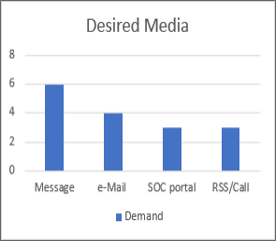
\includegraphics[scale=0.6]{Figures/product-media.png}
    \caption{Desired Media: Across available options}
    \label{fig:product-media}
\end{figure}
 \FloatBarrier
\textit{Messaging (Signal, WeChat)} 
is most preferred because the urgent issues having high risk can be communicated direct for immediate action.
\textit{e-Mail} is considered to be good for weekly communications on important cyber news items. 
With the \textit{SOC portal}, 
the items can be directly pushed to SOC dashboard. 
Other media like \textit{direct call} got importance in case of very urgent issues.
\textit{RSS} feed was the least desired media. 




\subsection{Desired Frequency}
\label{sec:frequency}
This was the reflection of the survey question number 13 and 14. We collected the desire about the frequency of cyber news items getting published to stakeholders 
according to FIGURE shown \ref{fig:stakeholder-problem-domain} in chapter \ref{Chapter4_problem-domain}, \nameref{Chapter4_problem-domain}. 

\begin{figure}[ht]
    \centering
    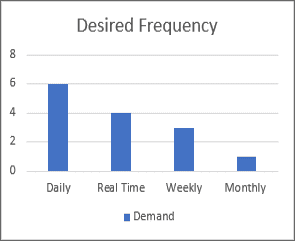
\includegraphics[scale=0.6]{Figures/product-frequency.png}
    \caption{Desired Frequency: Of the cyber newsfeed}
    \label{fig:product-frequency}
\end{figure}
 \FloatBarrier
Here is some interesting information provided by the Focus group.

\begin{itemize}
    \item Daily
        \begin{itemize}
            \item for direct important patches (e.g. Microsoft today)
            \item Daily feeds for information on cyber risks that require quick action
        \end{itemize}
    \item Others
        \begin{itemize}
            \item Actually as soon as it is available.
            \item real time, otherwise daily, depends a bit on the type of information
            \item Instant messages (e.g. using SMS etc) for High risk events
        \end{itemize}
    \item Weekly
        \begin{itemize}
            \item stay up to date info
            \item A weekly summary of the most relevant news (prioritized)
        \end{itemize}
    \item Monthly
        \begin{itemize}
            \item dashboard
            \item kpi's
            \item metrics
        \end{itemize}
\end{itemize}



\subsection{Willingness to Spend}
\label{sec:pay}
This was the reflection of the survey question number 17 and 18. The last input requested from the Focus group was about the willing to spend.  
The insight to this topic is very interesting as it can help the artefact to be productive and commercial.
\begin{figure}[ht]
    \centering
    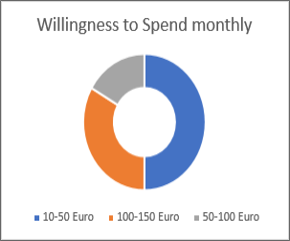
\includegraphics[scale=0.6]{Figures/product-cost.png}
    \caption{Cost of Cyber Intel produced by the  artefact}
    \label{fig:product-cost}
\end{figure}
 \FloatBarrier

\begin{itemize}
    \item 10-50 Euro
        \begin{itemize}
            \item is very much depending on how many users, 
            information wideness, 
            focused on the job element,
            measurements, 
            decision tree in it, etc.
            \item Very much depends on the size of the organisation and the environment. 
            As long as it is scalable, 
            or maybe as part of a larger services 
            (Network Operation Center (NOC) or SOC service).
        \end{itemize}
    \item 100-150 Euro
        \begin{itemize}
            \item 1200-1800 per year is a no brainer for companies and gives clearance in the overload in data
            \item Price will be determined by (demonstrated) value of information, but my guess would be that this is a good
introduction price. The higher the quality and relevance of information, the more this service give value to clients and
a higher price. It is all about the Return on Investment (ROI) that will be determined by the license model and value
        \end{itemize}
    \item 50-100 Euro
        \begin{itemize}
            \item This is dependant on the features, look and feel intuitiveness, and the possibilities I have to make the information
applicable and/or use it to make decisions.
        \end{itemize}
    
\end{itemize}



\section{Conclusion}
The GSS session turns out to be very productive and there were new insights discovered about the product on various parameters.  This concluded about the approach taken in this thesis to validate the artefact. Here we also shared the outcome of the discussions held during the GSS which we captured via an online survey tool.

